%
% Draft  document voiddocker.tex
%
 
\documentclass{article}  % Latex2e
\usepackage{graphicx,lscape,subfigure}
\usepackage[T1]{fontenc}
\usepackage{textcomp}
\usepackage{mathptmx}
\usepackage{listings}
\lstset{upquote=true,basicstyle={\small\ttfamily}}
 

\title{Making a docker image to run the Waterfox browser}
\author{Neville Jackson}
\date{4 Sep 2022} 

\begin{document} 

\maketitle      

\section{Introduction} 
This project is about learning how to compose a Dockerfile which runs an X11 application. The Waterfox browser was chosen as an example X11 application, because Waterfox is not available as a package in most Linux distributions, so the result might actually be a useful means of obtaining Waterfox without having to download a tarfile and do a local install. 

Getting a running Docker container to talk to the X11 server in the host system is relatively easy. Waterfox is a large and complex X application, and most of the challenge of this project is in setting up in the Docker image a working environmejnt for Waterfox. 

\section{What is involved in a normal Waterfox install?}
There is a document~\cite{wate:22a} on that.  Briefly the steps are
\begin{enumerate}
\item Download a tarfile from the Waterfox website~\cite{wate:22} or from the Github site~\cite{wate:22b}.
\item  Unpack the tarfile in /usr/local/src
\begin{verbatim}
bzip2 -dc waterfox-G4.1.1.1.en-US.linux-x86_64.tar.bz2 | tar xvf -
\end{verbatim}
\item Make a link in /usr/local/bin to point to the Waterfox binary
\begin{verbatim}
ln /usr/local/src/waterfox/waterfox /usr/local/bin/waterfox
\end{verbatim}
\item Define the desktop icon by adding a file waterfox.desktop to the directory /usr/share applications. The file waterfox.desktop does not come with the tarfile, but is available here~\cite{wate:22a}
\end{enumerate}
We need to implement steps 1 to 3 in a Dockerfile. Step 4 can be omitted, as there will be no icon if running Waterfox in a container. The container will have to be started from the command line.

\section{How to run a docker container requiring access to the host Xserver}
We assume the host is running X11 ( not Wayland ). Set up the following primitive Dockerfile.
\begin{verbatim}
FROM debian
WORKDIR /home/demo
RUN apt-get -y update
RUN apt-get -y upgrade
RUN apt-get -y x11-apps
RUN groupadd -g 1000 demo
RUN useradd -d /home/demo -s /bin/bash -m demo -u 1000 -g 1000
USER demo
ENV HOME /home/demo
CMD /usr/bin/xcalc
\end{verbatim}
 Build this with 
\begin{verbatim}
docker build -t nevj/test:v2 .
Sending build context to Docker daemon  2.048kB
Step 1/10 : FROM debian
 ---> 07d9246c53a6
Step 2/10 : WORKDIR /home/demo
 ---> Running in 2e0e40e0fd4c
..........
Successfully built 517c1937106a
Successfully tagged nevj/test:v2
\end{verbatim}
 Then run it with
\begin{verbatim}
[nevj@trinity dtest]$ xhost +
[nevj@trinity dtest]$ docker run -v /tmp/.X11-unix:/tmp/.X11-unix \
          -e DISPLAY=$DISPLAY -h $HOSTNAME \
          -v $HOME/.Xauthority:/home/nevj/.Xauthority nevj/test:v2
\end{verbatim}
and the xcalc app appears in a separate X window, as shown in Figure~\ref{fig:xcalc}
%\documentclass{article}
%\usepackage{graphicx,subfigure}
%\begin{document}

\begin{figure}[!h]
  \centering
   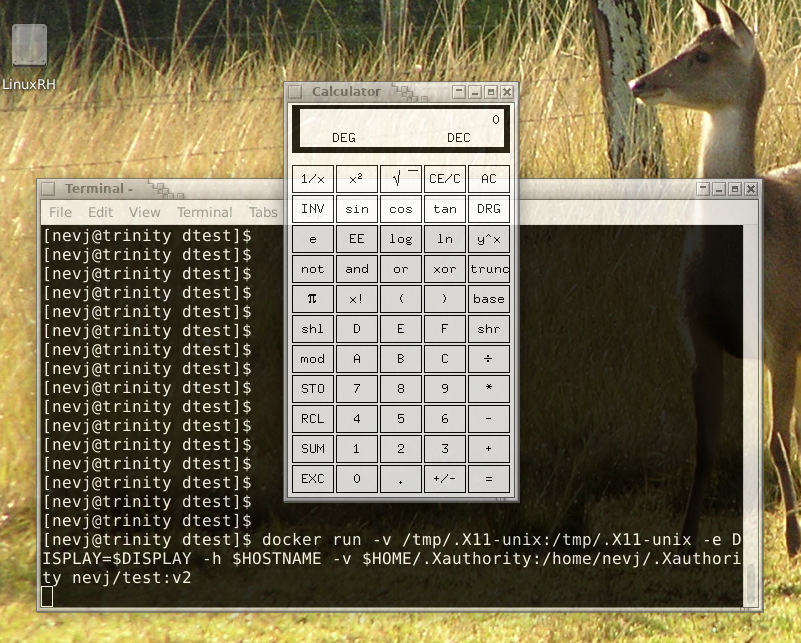
\includegraphics[width=0.9\textwidth]{xcalc.png}
  \caption{Xcalc app started from a Docker container}
  \label{fig:xcalc}
\end{figure}

%\end{document}


The {\em xhost +} statement is needed to give the container permission to communicate with the host X11 server. 
 The purpose of the options included in the {\em docker run} statement are as follows
\begin{description}
\item[-v /tmp/.X11-unix:/tmp/.X11-unix] defines a {\em mount} for a volume. The string {\em /tmp/.X11-unix:/tmp/.X11-unix} is the mount point on the host. The part before {\em ':'} is the volume name on the host. The part after {\em ':'} is where the file or directory is mounted oinside the container. A volume is just a file or directory in the host filesystem.
\item[-e DISPLAY=\$DISPLAY] sets the environment variable DISPLAY in the container
\item[-h \$HOSTNAME] sets the container hostname
\item[\$HOME/.Xauthority:/home/nevj/.Xauthority] sets the .Xauthority file of the container to the .Xauthority file of the host user who initiated the {\em run} statement again using a volume mount.
\item[nevj/test:v2] is the name of te image, build as above.
\end{description}
Volumes are the mechanism used by Docker containers to share data between the host and the container ( and between containers). They are need in this case because the container is an X11 client, while the host acts as the X11 server, so information has to pass between container and host.  A docker container can only write on the part of the host filesystem defined as a docker volume. There is also {\em tmpfs mount} which is a temporary ram disk used for non-permanent data within a container.

\section{First attempt at a Waterfox Dockerfile, using a  Debian parent image}
There is no new principle involved in running Waterfox rather than the simple xcalc app, in a docker container. The Waterfox browser is a large program with many dependencies, so the Dockerfile will have to build up a complete working environment specifically for Waterfox. 

I chose Debian parent image for a first attempt, because Debian is familiar and is most likely to compatable with Waterfox.  The Debian parent image is large. We shall try later to repeat the job with a smaller parent image. 

\subsection{Finding the dependencies of a binary program file}
There is a really good article~\cite{rehn:21} on identifying dependencies of a runtime binary when making a dockerfile.

If one looks at the unpacked Waterfox ditribution tarfile, it contains the files shon in Figure~\ref{fig:wfoxfiles}
%\documentclass{article}
%\usepackage{graphicx,subfigure}
%\begin{document}

\begin{figure}[!h]
  \centering
   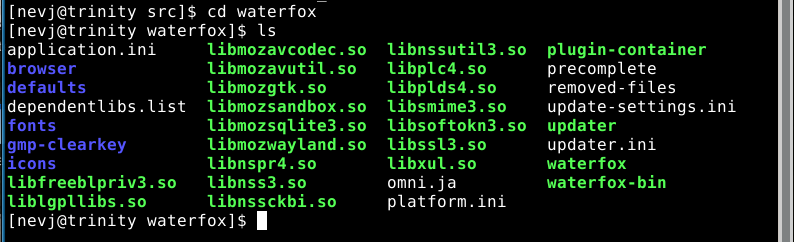
\includegraphics[width=0.9\textwidth]{wfoxfiles.png}
  \caption{Files contained in the waterfox distribution tarfile}
  \label{fig:wfoxfiles}
\end{figure}

%\end{document}


The *.so files shown in green are dynamically loaded libraries. Presumably these are all dependencies of waterfox, but they may not be the only dependencies. There is a file TwemojiMozilla.ttf in the fonts subdirectory, and there are various default configuration files.

An initial check for dependencies can be obtained with {\em ldd}
\begin{verbatim}
nevj@mary:/usr/local/src/waterfox$ ldd waterfox
	linux-vdso.so.1 (0x00007ffc3eb95000)
	libpthread.so.0 => /lib/x86_64-linux-gnu/libpthread.so.0 (0x00007f2a6d46c000)
	libdl.so.2 => /lib/x86_64-linux-gnu/libdl.so.2 (0x00007f2a6d466000)
	libstdc++.so.6 => /lib/x86_64-linux-gnu/libstdc++.so.6 (0x00007f2a6d299000)
	libm.so.6 => /lib/x86_64-linux-gnu/libm.so.6 (0x00007f2a6d155000)
	libgcc_s.so.1 => /lib/x86_64-linux-gnu/libgcc_s.so.1 (0x00007f2a6d13b000)
	libc.so.6 => /lib/x86_64-linux-gnu/libc.so.6 (0x00007f2a6cf76000)
	/lib64/ld-linux-x86-64.so.2 (0x00007f2a6d569000)
\end{verbatim}
This is best done in a Debian system in which waterfox has been installed
There are 8 libraries called directly by waterfox, and none of them are present in the distribution tarfile. These are libraries required for waterfox to start up. Note that linux-vdso.so.1 is a virtual library, ie it is built into the kernel and does not exist as a package. The other 7 should each be supplied by a package. We shall leave the problem of finding the package names which supply each library later.

 There may also be libraries which waterfoox loads dynamically while executing. To find these we do the following, again in a Debian system
\begin{verbatim}
nevj@mary:~$ LD_DEBUG=libs waterfox >&logfile

nevj@mary:~$ cat logfile
     2572:     find library=libpthread.so.0 [0]; searching
      2572:      search cache=/etc/ld.so.cache
      2572:       trying file=/lib/x86_64-linux-gnu/libpthread.so.0
      2572:
      2572:     find library=libdl.so.2 [0]; searching
      2572:      search cache=/etc/ld.so.cache
      2572:       trying file=/lib/x86_64-linux-gnu/libdl.so.2
      2572:
      2572:     find library=libstdc++.so.6 [0]; searching
      2572:      search cache=/etc/ld.so.cache
      2572:       trying file=/lib/x86_64-linux-gnu/libstdc++.so.6
      2572:
      2572:     find library=libm.so.6 [0]; searching
      2572:      search cache=/etc/ld.so.cache
      2572:       trying file=/lib/x86_64-linux-gnu/libm.so.6
      2572:
      2572:     find library=libgcc_s.so.1 [0]; searching
      2572:      search cache=/etc/ld.so.cache
      2572:       trying file=/lib/x86_64-linux-gnu/libgcc_s.so.1
     2572:
      2572:     find library=libc.so.6 [0]; searching
      2572:      search cache=/etc/ld.so.cache
      2572:       trying file=/lib/x86_64-linux-gnu/libc.so.6
      2572:
      2572:
      2572:     calling init: /lib/x86_64-linux-gnu/libpthread.so.0
      2572:
      2572:
      2572:     calling init: /lib/x86_64-linux-gnu/libc.so.6
      2572:
      2572:
      2572:     calling init: /lib/x86_64-linux-gnu/libgcc_s.so.1
      2572:
      2572:
      2572:     calling init: /lib/x86_64-linux-gnu/libm.so.6
      2572:
      2572:
      2572:     calling init: /lib/x86_64-linux-gnu/libstdc++.so.6
      2572:
      2572:
      2572:     calling init: /lib/x86_64-linux-gnu/libdl.so.2
      2572:
      2572:
      2572:     initialize program: waterfox
      2572:
      2572:
      2572:     transferring control: waterfox
      2572:
      2572:
      2572:     calling init: /usr/local/src/waterfox/libnspr4.so
      2572:
      2572:
      2572:     calling init: /usr/local/src/waterfox/libplc4.so
      2572:
      2572:
      2572:     calling init: /usr/local/src/waterfox/libplds4.so
      2572:
      2572:     find library=librt.so.1 [0]; searching
      2572:      search cache=/etc/ld.so.cache
      2572:       trying file=/lib/x86_64-linux-gnu/librt.so.1
      2572:
      2572:
      2572:     calling init: /lib/x86_64-linux-gnu/librt.so.1
      2572:
      2572:
      2572:     calling init: /usr/local/src/waterfox/libmozsandbox.so
      2572:
      2572:
      2572:     calling init: /usr/local/src/waterfox/liblgpllibs.so
      2572:
      2572:
      2572:     calling init: /usr/local/src/waterfox/libnssutil3.so
      2572:
      2572:
      2572:     calling init: /usr/local/src/waterfox/libnss3.so
      2572:
  ..................
     2796:     calling init: /lib/x86_64-linux-gnu/libX11-xcb.so.1
      2796:
      2796:
      2796:     calling init: /usr/local/src/waterfox/libxul.so
      2796:
      2796:     /usr/local/src/waterfox/waterfox: error: symbol lookup error:
 undefined symbol: nspr_use_zone_allocator (fatal)
      2796:
      2796:     calling init: /usr/local/src/waterfox/libsoftokn3.so
      2796:
      2796:
      2796:     calling init: /usr/local/src/waterfox/libfreeblpriv3.so
      2796:
JavaScript error: resource://gre/modules/PartitioningExceptionListService.jsm
, line 69: NS_ERROR_MALFORMED_URI: Component returned failure code: 0x804b000
a (NS_ERROR_MALFORMED_URI) [nsIPartitioningExceptionListObserver.onExceptionL
istUpdate]
console.error: PushService:
  clearOriginData: Error clearing origin data:
  TypeError
JavaScript error: resource:///modules/Interactions.jsm, line 209: NS_ERROR_FA
ILURE: Component returned failure code: 0x80004005 (NS_ERROR_FAILURE) [nsIUse
rIdleService.removeIdleObserver]

###!!! [Parent][RunMessage] Error: Channel closing: too late to send/recv, me
ssages will be lost
\end{verbatim}
Lots of messages, had to truncate it, was 5744 lines.
The first 3 lines say it is searching for a system library called {\em libpthread}. The lines beginning {\em calling init} indicate the library has been found and give its absolute path. Some libraries may not be found, and they will have no line beginning {\em calling init}. We can get a list of libraries found with 
\begin{verbatim}
nevj@mary:~$  cat out | grep init > outinit
nevj@mary:~$ wc outinit
  715  2878 45875 outinit
nevj@mary:~$  cat outinit
   2572:	calling init: /lib/x86_64-linux-gnu/libpthread.so.0
      2572:	calling init: /lib/x86_64-linux-gnu/libc.so.6
      2572:	calling init: /lib/x86_64-linux-gnu/libgcc_s.so.1
      2572:	calling init: /lib/x86_64-linux-gnu/libm.so.6
      2572:	calling init: /lib/x86_64-linux-gnu/libstdc++.so.6
      2572:	calling init: /lib/x86_64-linux-gnu/libdl.so.2
      2572:	initialize program: waterfox
      2572:	calling init: /usr/local/src/waterfox/libnspr4.so
      2572:	calling init: /usr/local/src/waterfox/libplc4.so
      2572:	calling init: /usr/local/src/waterfox/libplds4.so
      2572:	calling init: /lib/x86_64-linux-gnu/librt.so.1
      2572:	calling init: /usr/local/src/waterfox/libmozsandbox.so
      2572:	calling init: /usr/local/src/waterfox/liblgpllibs.so
      2572:	calling init: /usr/local/src/waterfox/libnssutil3.so
      2572:	calling init: /usr/local/src/waterfox/libnss3.so
      2572:	calling init: /usr/local/src/waterfox/libsmime3.so
      2572:	calling init: /usr/local/src/waterfox/libmozsqlite3.so
      2572:	calling init: /usr/local/src/waterfox/libssl3.so
      2572:	calling init: /lib/x86_64-linux-gnu/libgpg-error.so.0
  ............
\end{verbatim}
  
So there are still 715 of them. The first 6 are the startiup dependencies, and the rest are runtime dependencies

There is also the question of configuration files. Most of these are hopefully included in the Waterfox tarfile. We can check
\begin{verbatim}
strace --trace=open,openat /usr/local/bin/waterfox >&strace.out

Lots of libraries which we can ignore
....
Conf files
openat(AT_FDCWD, "/etc/host.conf", O_RDONLY|O_CLOEXEC) = 7
openat(AT_FDCWD, "/etc/resolv.conf", O_RDONLY|O_CLOEXEC) = 7
openat(AT_FDCWD, "/etc/nsswitch.conf", O_RDONLY|O_CLOEXEC) = 7
openat(AT_FDCWD, "/etc/ld.so.cache", O_RDONLY|O_CLOEXEC) = 7
......
openat(AT_FDCWD, "/home/nevj/.Xauthority", O_RDONLY) = 5
openat(AT_FDCWD, "/usr/share/X11/locale/locale.alias", O_RDONLY) = 5
openat(AT_FDCWD, "/usr/share/X11/locale/locale.alias", O_RDONLY) = 5
openat(AT_FDCWD, "/usr/share/X11/locale/locale.dir", O_RDONLY) = 5
openat(AT_FDCWD, "/usr/share/X11/locale/en_US.UTF-8/XLC_LOCALE", O_RDONLY) = 
5
openat(AT_FDCWD, "/home/nevj/.Xdefaults-mary", O_RDONLY) = -1 ENOENT (No such
 file or directory)
....
openat(AT_FDCWD, "/home/nevj/.waterfox/profiles.ini", O_RDONLY) = 8
openat(AT_FDCWD, "/home/nevj/.Xauthority", O_RDONLY) = 9
....
openat(AT_FDCWD, "/usr/local/src/waterfox/omni.ja", O_RDONLY) = 14
openat(AT_FDCWD, "/usr/local/src/waterfox/browser/omni.ja", O_RDONLY) = 15
openat(AT_FDCWD, "/sys/devices/system/cpu", O_RDONLY|O_NONBLOCK|O_CLOEXEC|O_D
IRECTORY) = 16
openat(AT_FDCWD, "/usr/local/src/waterfox/defaults/pref", O_RDONLY|O_NONBLOCK
|O_CLOEXEC|O_DIRECTORY) = 16
openat(AT_FDCWD, "/usr/local/src/waterfox/defaults/pref/channel-prefs.js", O_
RDONLY) = 17
......
openat(AT_FDCWD, "/usr/share/fontconfig/conf.avail/11-lcdfilter-default.conf"
, O_RDONLY|O_CLOEXEC) = 38
openat(AT_FDCWD, "/etc/fonts/conf.avail/20-unhint-small-dejavu-lgc-sans-mono.
conf", O_RDONLY|O_CLOEXEC) = 38
.....
openat(AT_FDCWD, "/etc/os-release", O_RDONLY) = 37
openat(AT_FDCWD, "/sys/devices/system/cpu/present", O_RDONLY) = 37
openat(AT_FDCWD, "/usr/share/locale/locale.alias", O_RDONLY) = 38
openat(AT_FDCWD, "/usr/share/icons/Tango/index.theme", O_RDONLY) = 38
openat(AT_FDCWD, "/usr/share/icons/Tango/icon-theme.cache", O_RDONLY) = 38
......
openat(AT_FDCWD, "/usr/share/icons/index.theme", O_RDONLY) = -1 ENOENT (No su
ch file or directory)
openat(AT_FDCWD, "/usr/share/pixmaps/cursors/e-resize", O_RDONLY) = -1 ENOENT
 (No such file or directory)
....
penat(AT_FDCWD, "/home/nevj/.icons/Adwaita/cursors/e-resize", O_RDONLY) = -1
 ENOENT (No such file or directory)
openat(AT_FDCWD, "/home/nevj/.icons/Adwaita/index.theme", O_RDONLY) = -1 ENOE
NT (No such file or directory)
.....
openat(AT_FDCWD, "/home/nevj/.config/xfce-mimeapps.list", O_RDONLY) = -1 ENOE
NT (No such file or directory)
openat(AT_FDCWD, "/home/nevj/.config/mimeapps.list", O_RDONLY) = 80
....
openat(AT_FDCWD, "/usr/local/share/applications/xfce-mimeapps.list", O_RDONLY
) = -1 ENOENT (No such file or directory)
openat(AT_FDCWD, "/usr/local/share/applications/mimeapps.list", O_RDONLY) = -
1 ENOENT (No such file or directory)
openat(AT_FDCWD, "/usr/local/share/applications/defaults.list", O_RDONLY) = -
1 ENOENT (No such file or directory)
openat(AT_FDCWD, "/usr/local/share/applications/mimeinfo.cache", O_RDONLY) = 
-1 ENOENT (No such file or directory)
.....
openat(AT_FDCWD, "/usr/share/fonts/truetype/dejavu/DejaVuSans-Bold.ttf", O_RD
ONLY) = 88
JavaScript error: resource:///actors/AboutNewTabParent.jsm, line 23: InvalidS
tateError: An attempt was made to use an object that is not, or is no longer,
 usable
.....
JavaScript error: resource://gre/modules/PartitioningExceptionListService.jsm
, line 69: NS_ERROR_MALFORMED_URI: Component returned failure code: 0x804b000
a (NS_ERROR_MALFORMED_URI) [nsIPartitioningExceptionListObserver.onExceptionL
istUpdate]
....
penat(AT_FDCWD, "/home/nevj/.icons/Adwaita/cursors/hand2", O_RDONLY) = -1 EN
OENT (No such file or directory)
openat(AT_FDCWD, "/home/nevj/.icons/Adwaita/index.theme", O_RDONLY) = -1 ENOE
NT (No such file or directory)
.....
\end{verbatim}
 Some of the files have the message {\em (No such file or directory)}. They are probably not serious issues... the above was done in a Waterfox install which works satisfactorily. I have only shown a selection. The full output above was 1402 lines. 


\subsection{Which Debian packages provide these files?}
We have a long list of files which are dependencies. We need to convert this into a list of {\em .deb} packages which supply the necessary files.  That should reduce the information to a much shorter list of packages. The tool for finding which package supplies a file is {\em apt-file}.

{\em apt-file} is not part of a standard Debian system. We need to install it

\begin{verbatim}
root@trinity:/home/nevj# apt-get install apt-file
......
The following additional packages will be installed:
  libapt-pkg-perl libexporter-tiny-perl liblist-moreutils-perl
  liblist-moreutils-xs-perl libregexp-assemble-perl
The following NEW packages will be installed:
  apt-file libapt-pkg-perl libexporter-tiny-perl liblist-moreutils-perl
  liblist-moreutils-xs-perl libregexp-assemble-perl
0 upgraded, 6 newly installed, 0 to remove and 6 not upgraded.
Need to get 322 kB of archives.
After this operation, 901 kB of additional disk space will be used.
The following additional packages will be installed:
  libapt-pkg-perl libexporter-tiny-perl liblist-moreutils-perl
  liblist-moreutils-xs-perl libregexp-assemble-perl
The following NEW packages will be installed:
  apt-file libapt-pkg-perl libexporter-tiny-perl liblist-moreutils-perl
  liblist-moreutils-xs-perl libregexp-assemble-perl
0 upgraded, 6 newly installed, 0 to remove and 6 not upgraded.
Need to get 322 kB of archives.
After this operation, 901 kB of additional disk space will be used.
The following additional packages will be installed:
  libapt-pkg-perl libexporter-tiny-perl liblist-moreutils-perl
  liblist-moreutils-xs-perl libregexp-assemble-perl
The following NEW packages will be installed:
  apt-file libapt-pkg-perl libexporter-tiny-perl liblist-moreutils-perl
  liblist-moreutils-xs-perl libregexp-assemble-perl
0 upgraded, 6 newly installed, 0 to remove and 6 not upgraded.
Need to get 322 kB of archives.
After this operation, 901 kB of additional disk space will be used.
The following additional packages will be installed:
  libapt-pkg-perl libexporter-tiny-perl liblist-moreutils-perl
  liblist-moreutils-xs-perl libregexp-assemble-perl
The following NEW packages will be installed:
  apt-file libapt-pkg-perl libexporter-tiny-perl liblist-moreutils-perl
  liblist-moreutils-xs-perl libregexp-assemble-perl
0 upgraded, 6 newly installed, 0 to remove and 6 not upgraded.
Need to get 322 kB of archives.
After this operation, 901 kB of additional disk space will be used.
The following additional packages will be installed:
  libapt-pkg-perl libexporter-tiny-perl liblist-moreutils-perl
  liblist-moreutils-xs-perl libregexp-assemble-perl
The following NEW packages will be installed:
  apt-file libapt-pkg-perl libexporter-tiny-perl liblist-moreutils-perl
  liblist-moreutils-xs-perl libregexp-assemble-perl
0 upgraded, 6 newly installed, 0 to remove and 6 not upgraded.
Need to get 322 kB of archives.
After this operation, 901 kB of additional disk space will be used.
......
\end{verbatim}
Then we need to generate apt-file's database
\begin{verbatim}
root@trinity:/home/nevj# apt-file update
\end{verbatim}
Then we can search 
\begin{verbatim}
nevj@trinity:~$ apt-file search libpthread.so.0
libc6: /lib/x86_64-linux-gnu/libpthread.so.0
......
Lots of other libraries .... it is better to use dthe full path
nevj@trinity:~$ apt-file search /lib/x86_64-linux-gnu/libpthread.so.0
libc6: /lib/x86_64-linux-gnu/libpthread.so.0
 So we just get the relevant one
\end{verbatim}


There is an alternative to apt-file
\begin{verbatim}
nevj@trinity:~$ dpkg -s libpthread.so.0
dpkg-query: package 'libpthread.so.0' is not installed and no information is available
Use dpkg --info (= dpkg-deb --info) to examine archive files.
\end{verbatim}
 So {\em dpkg -s} only works for installed library files, {\em apt-file works for all available packages}.

Now we have the tools , it is a mere matter of feeding several hundred library files to {\em apt-file search} . 
\begin{verbatim}
#  a bit of hand editing
$  cp outinit outinit.edit
$  vi outinit.edit

# make a simple awk script to extract the 4th field
$ vi field4.awk
{print $4}

# run the script
$ awk -f field4.awk < outinit.edit > libfiles.txt

# and the output is
$ more libfiles.txt
/lib/x86_64-linux-gnu/libpthread.so.0
/lib/x86_64-linux-gnu/libc.so.6
/lib/x86_64-linux-gnu/libgcc_s.so.1
/lib/x86_64-linux-gnu/libm.so.6
/lib/x86_64-linux-gnu/libstdc++.so.6
/lib/x86_64-linux-gnu/libdl.so.2
/usr/local/src/waterfox/libnspr4.so
/usr/local/src/waterfox/libplc4.so
....... too many to list

  $ wc libfiles.txt
  711   711 26829 libfiles.txt
So 711 libraries in total
\end{verbatim}
  So now we have out list of libraries,  we need a shell script to feed it to apt-file.
\begin{lstlisting}
#! /bin/csh
foreach lib (`cat libfiles.txt`)
 apt-file --fixed-string -l search $lib >>& package.txt
end
\end{lstlisting}
Now if we run that script we get
\begin{verbatim}
chmod 755 packages.csh
./packages.csh
wc package.txt
 125  125 1124 package.txt
\end{verbatim}
So we have reduced from 711 libraries  to 125 packages. However there are duplicates so
\begin{verbatim}
sort <package.txt | uniq >uniqpackage.txt
wc uniqpackage.txt
 21  21 249 uniqpackage.txt
cat uniqpackage.txt
dconf-gsettings-backend
gvfs
gvfs-libs
libc6
libcom-err2
libdbus-1-3
libelogind0
libexpat1
libgcc-s1
libgdk-pixbuf-2.0-0
libgl1-mesa-dri
libgpg-error0
libkeyutils1
liblzma5
libnss-mdns
libpcre3
libpulse0
libselinux1
libtirpc3
python3-minimal
zlib1g
\end{verbatim}
 There are 21 unique packages reguired.
Now we can write the Dockerfile with some confidence that it will supply an suitable environment for Waterfox.

\subsection{First Debian parent Dockerfile}
For a first attempt, we will use a copy of the waterfox tarfile which I have downloaded and placed in the Dockerfile directory. Later we will try to setup the Dockerfile to download it from the Waterfox site~\cite{wate:22b}.

We will work within the container in a directory {\em /wfox}. There will be a user called {\em wfox} and the container will execute the waterfox binary.

Our first Dockerfile is as follows
\begin{verbatim}
# get a parent image
FROM debian:stable-20220801

#set working dir inside container
WORKDIR /wfox

# get waterfox
COPY . .

# install waterfox.desktop file
RUN mkdir /usr/share/applications && \
  cp waterfox.desktop /usr/share/applications

#  
RUN cd /etc/apt && \
# apt debian setup
  cp sources.list sources.list.orig && \
  sed 's/main/main contrib non-free/' sources.list.orig >sources.list && \
  cd /wfox && \
  apt-get update && \
  apt-get upgrade -y && \
# apt install libraries
  apt-get install -y  dconf-gsettings-backend gvfs gvfs-libs libc6 libcom-err2 libdbus-1-3 libelogind0 libexpat1 libgcc-s1 libgdk-pixbuf-2.0-0 libgl1-mesa-dri libgpg-error0 libkeyutils1 liblzma5 libnss-mdns libpcre3 libpulse0 libselinux1 libtirpc3 python3-minimal zlib1g

#    unpack waterfox distro tarfile
  cd /wfox && \
  bzip2 -dc waterfox-G4.1.4.en-US.linux-x86_64.tar.bz2 | tar xvf - 
# setup environment
RUN groupadd -g 1000 wfox
RUN useradd -d /home/wfox -s /bin/bash -m wfox -u 1000 -g 1000
USER wfox
ENV HOME /home/wfox
CMD /wfox/waterfox/waterfox
\end{verbatim}
 Then build an image using the above Dockerfile and run it
\begin{verbatim}
# work directory in host system
cd ~/Waterfox.docker
ls
Dockerfile  junk      waterfox-G4.1.4.en-US.linux-x86_64.tar.bz2  wget
buildrun    libsused  waterfox.desktop                            x11docker

# docker build
docker build -t wfoxdeb:v1 .
.....
Successfully built 7d1e1798583a
Successfully tagged wfoxdeb:v1

#docker run
docker run -v /tmp/.X11-unix:/tmp/.X11-unix -e DISPLAY=$DISPLAY -h $HOSTNAME -v $HOME/.Xauthority:/home/nevj/.Xauthority xfoxdeb:v1

XPCOMGlueLoad error for file /wfox/waterfox/libmozgtk.so:
libgtk-3.so.0: cannot open shared object file: No such file or directory
Couldn't load XPCOM.
\end{verbatim}
 What the message means is that the library {\em libmozgtk.so} which comes with the waterfox tarfile requires the library {\em libgtk-3.so.0}, but it was not present in the container system.

So our wonderful, complicated procedure for reducing 711 libraries to 21 packages has missed something. What is missing is that we traced all the libraries called by the {\em waterfox} binary, but we neglected to trace all the libraries called by the 18 special waterfox libraries included in the waterfox tarfile. 

We need to do the library tracing and package finding all over again for each of the 18 special libraries. 

\subsection{Dependencies of the 18 special {\em waterfox} libraries.}
We setup a list of the 18 special libraries in a file {\em list18libs.txt}. We need to process each library in the list with {\em ldd} so we setup a script. We can not execute a library, so we cant use {\em strace} or {\em LD\_DEBUG} , but we can use {\em ldd}.
\begin{verbatim}
cd /usr/local/src/waterfox
ls | grep so 
libfreeblpriv3.so
liblgpllibs.so
libmozavcodec.so
libmozavutil.so
libmozgtk.so
libmozsandbox.so
libmozsqlite3.so
libmozwayland.so
libnspr4.so
libnss3.so
libnssckbi.so
libnssutil3.so
libplc4.so
libplds4.so
libsmime3.so
libsoftokn3.so
libssl3.so
libxul.so
\end{verbatim}

 Store this on a file
\begin{lstlisting}
ls | grep so > list18libs.txt
# make a script to process each of these with ldd
#! /bin/csh
foreach lib (`cat list18libs.txt`)
  ldd lib >>& list18libsdeps.txt
end
\end{lstlisting}

How many libraries found?
\begin{verbatim} 
wc list18libsdeps.txt
  291  1107 20639 list18libsdeps.txt
\end{verbatim}
What packages contain these libraries?
t have a look at list18libsdeps.txt
\begin{verbatim}
head list18libsdeps.txt
	linux-vdso.so.1 (0x00007fff591c5000)
	libpthread.so.0 => /lib/x86_64-linux-gnu/libpthread.so.0 (0x00007f346a0d9000)
	libnspr4.so => /lib/x86_64-linux-gnu/libnspr4.so (0x00007f346a098000)
	libplc4.so => /lib/x86_64-linux-gnu/libplc4.so (0x00007f346a091000)
	libplds4.so => /lib/x86_64-linux-gnu/libplds4.so (0x00007f346a08c000)
	libdl.so.2 => /lib/x86_64-linux-gnu/libdl.so.2 (0x00007f346a086000)
	libc.so.6 => /lib/x86_64-linux-gnu/libc.so.6 (0x00007f3469ec1000)
	/lib64/ld-linux-x86-64.so.2 (0x00007f346a1eb000)
	linux-vdso.so.1 (0x00007ffec61a5000)
	libpthread.so.0 => /lib/x86_64-linux-gnu/libpthread.so.0 (0x00007ffaa2b5d000)
......
\end{verbatim}
We need the third field from the file list18libsdeps.txt, so use our awk script again, after removing the first line
\begin{verbatim}
cat field3.awk
{print $3}

awk -f field3.awk <list18libsdeps.txt2 >list18libsdeps.txt3
head list18libsdeps.txt3
/lib/x86_64-linux-gnu/libpthread.so.0
/lib/x86_64-linux-gnu/libnspr4.so
/lib/x86_64-linux-gnu/libplc4.so
/lib/x86_64-linux-gnu/libplds4.so
/lib/x86_64-linux-gnu/libdl.so.2
/lib/x86_64-linux-gnu/libc.so.6


/lib/x86_64-linux-gnu/libpthread.so.0
/lib/x86_64-linux-gnu/libdl.so.2
.......
\end{verbatim}
We have extracted the full pathname of each library, there are a few blank line, so we edit those out (may not actually matter, then
\begin{verbatim}
wc list18libsdeps.txt3
 245  245 8897 list18libsdeps.txt3
\end{verbatim}
There are 245 library paths left. We can process this with {\em apt-file} to see what packages supply these libraries
\begin{verbatim}
cat packages18.csh
#! /bin/csh
foreach lib (`cat list18libsdeps.txt3`)
 apt-file --fixed-string -l search $lib >>& package18.txt
end

./packages18.

wc package18.txt
 85  85 596 package18.txt

head package18.txt
libc6
libc6
libc6
libc6
libc6
libc6
libgcc-s1
libc6
libc6
libc6
......
\end{verbatim}
We have reduced te 245 library paths to 85 packages, but we can see from the partial listing there are lots of duplicates, so
\begin{verbatim}
sort package18.txt | uniq > uniqpackage18.txt
wc uniqpackage18.txt
 10  10 101 uniqpackage18.txt
cat uniqpackage18.txt
libc6
libdbus-1-3
libelogind0
libexpat1
libgcc-s1
libgpg-error0
liblzma5
libpcre3
libselinux1
zlib1g
\end{verbatim}
 There are 10 unique package names, and all 10 are already present in our previous list of 21 required packages.  So this does not solve the dependency problem ?

An investigation of each of the above steps reveals that the {\em apt-file} statement in the script packages18.csh does not require the option {\em --fixed-string}. Running this step again leads to

\begin{verbatim}
cat packages18.csh
#! /bin/csh
foreach lib (`cat list18libsdeps.txt3`)
 apt-file  -l search $lib >>& package18.txt
end

./packages18.chh

wc package18.txt
 338  338 3128 package18.txt

\end{verbatim}
So now we have 338 packages instead of 245. Removing duplicates again gives
\begin{verbatim}
sort package18.txt | uniq >uniqpackage18.txt

wc uniqpackage18.txt
 72  72 853 uniqpackage18.txt

head uniqpackage18.txt
libatk1.0-0
libatk-bridge2.0-0
libatspi2.0-0
libblkid1
libbrotli1
libbsd0
libc6
libcairo2
libcairo-gobject2
libdatrie1
......
\end{verbatim}

We now have 72 package some of which  are not included in  the 21  package dependencies of the waterfox binary. We need to remove from these 72 those which are  in both lists
\begin{verbatim}
sort uniqpackage.txt > sorteduniqpackage.txt
sort uniqpackage18.txt > sorteduniqpackage18.txt
comm -3 sorteduniqpackage.txt sorteduniqpackage18.txt >commpackage.txt

wc commpackage.txt
 71  71 921 commpackage.txt
\end{verbatim}
So we still have 71 packages to add to the Dockerfile.

\subsection{Second Debian parent Dockerfile attempt}
We now add an apt-get install for the 71 packages required to satisfy Waterfox's 18 special libraries. So version 2 of our Dockerfile looks as follows
\begin{verbatim}

FROM debian:stable-20220801
#set working dir inside container
WORKDIR /wfox
# get waterfox
COPY . .
# install waterfox.desktop file
RUN mkdir /usr/share/applications && \
  cp waterfox.desktop /usr/share/applications
#
RUN cd /etc/apt && \
# apt debian setup
  cp sources.list sources.list.orig && \
  sed 's/main/main contrib non-free/' sources.list.orig >sources.list && \
  cd /wfox && \
  apt-get update && \
  apt-get upgrade -y && \
# apt install packages for waterfox
  apt-get install -y  dconf-gsettings-backend gvfs gvfs-libs libc6 libcom-err2 libdbus-1-3 libelogind0 libexpat1 libgcc-s1 libgdk-pixbuf-2.0-0 libgl1-mesa-dri libgpg-error0 libkeyutils1 liblzma5 libnss-mdns libpcre3 libpulse0 libselinux1 libtirpc3 python3-minimal zlib1g && \
# apt install packages for waterfox libraries
  apt-get install -y libatk1.0-0 libatk-bridge2.0-0 libatspi2.0-0 libblkid1 libbrotli1 libbsd0 libc6 libcairo2 libcairo-gobject2 libdatrie1 libdbus-1-3 libdbus-glib-1-2 libelogind0 libepoxy0 libexpat1 libffi7 libfontconfig1 libfreetype6 libfribidi0 libgcc-s1 libgcrypt20 libgdk-pixbuf-2.0-0 libglib2.0-0 libglib2.0-dev libgpg-error0 libgraphite2-3 libgtk-3-0 libharfbuzz0b libice6 liblz4-1 liblzma5 libmd0 libmount1 libnspr4 libnss3 libpango-1.0-0 libpangocairo-1.0-0 libpangoft2-1.0-0 libpcre2-8-0 libpcre3 libpixman-1-0 libpng16-16 libselinux1 libsm6 libstdc++6 libsystemd0 libthai0 libuuid1 libwayland-client0 libwayland-cursor0 libwayland-egl1 libx11-6 libx11-xcb1 libxau6 libxcb1 libxcb-render0 libxcb-shm0 libxcomposite1 libxcursor1 libxdamage1 libxdmcp6 libxext6 libxext6-dbg libxfixes3 libxi6 libxinerama1 libxkbcommon0 libxrandr2 libxrender1 libxt6 libzstd1 zlib1g && \
# needed to unpack waterfox tarfile
 apt-get install -y bzip2 && \
#    unpack waterfox distro tarfile
  cd /wfox && \
  bzip2 -dc waterfox-G4.1.4.en-US.linux-x86_64.tar.bz2 | tar xvf -
# setup environment
RUN groupadd -g 1000 wfox
RUN useradd -d /home/wfox -s /bin/bash -m wfox -u 1000 -g 1000
USER wfox
ENV HOME /home/wfox
# exec waterfox
CMD /wfox/waterfox/waterfox
\end{verbatim}
We build this Dockerfile with
\begin{verbatim}
docker build -t wfoxdeb:vt2 .
\end{verbatim}
and it fails to build because the packages libelogind0 and libsystemd0 have conflicts and apt refuses to install both. We choose to delete libelogind0. 
Then the build works , and we are able to run its docker image with
\begin{verbatim}
xhost +
docker run -v /tmp/.X11-unix:/tmp/.X11-unix -e DISPLAY=$DISPLAY -h $HOSTNAME -v $HOME/.Xauthority:/home/nevj/.Xauthority wfoxdeb:vt2
\end{verbatim}
This time we are successful. The container executes the Waterfox binary and we ger an X11 window with a blank welcome page shown in Figure~\ref{fig:welcom}, a correct release page shown in Figure~\ref{fig:releas}, all the search functions and page displays seem to work as shown in Figure~\ref{fig:search}
%\documentclass{article}
%\usepackage{graphicx,subfigure}
%\begin{document}

\begin{figure}[!h]
  \centering
   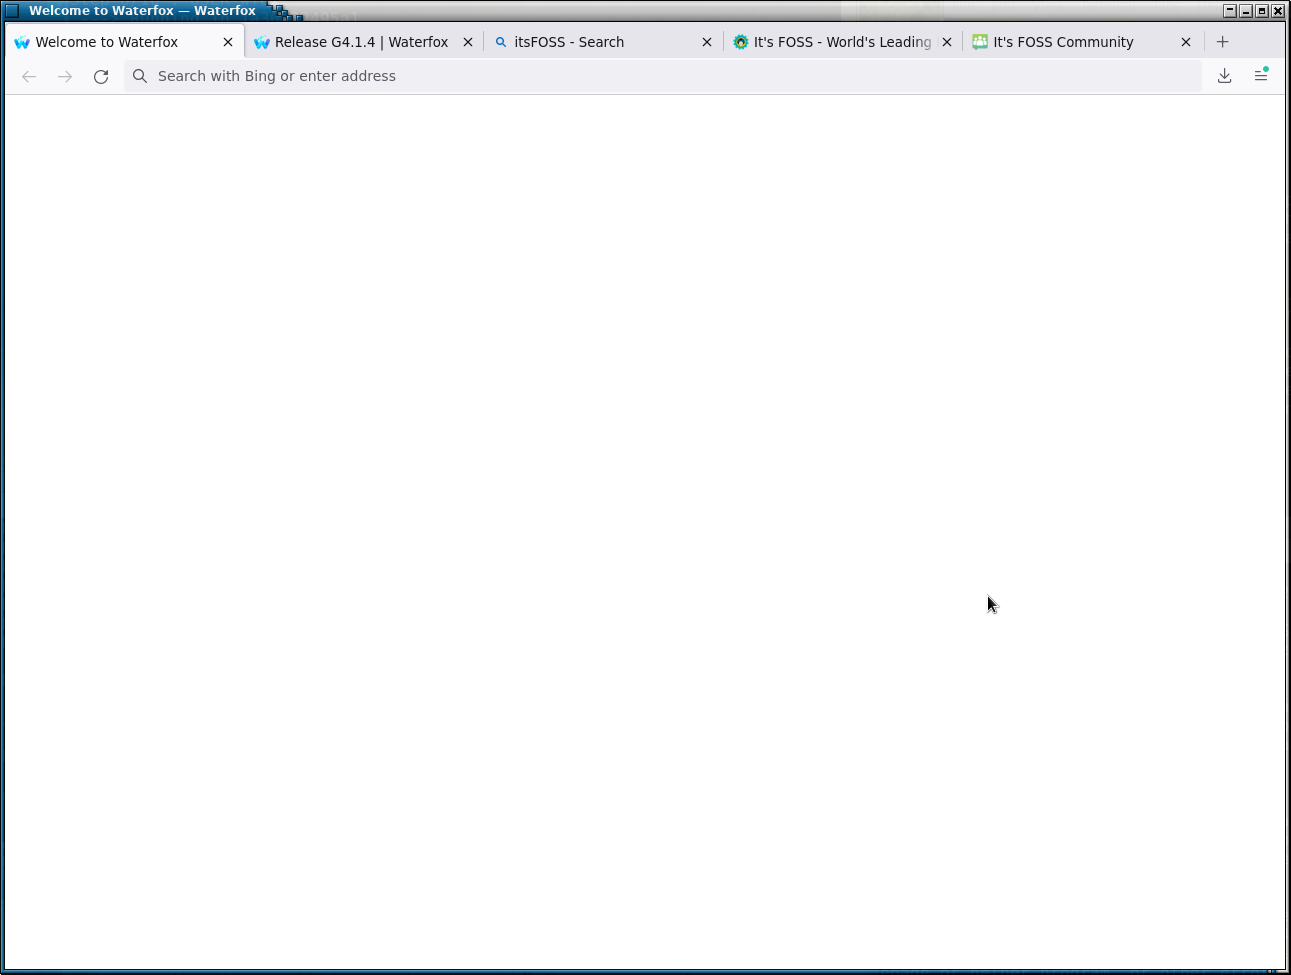
\includegraphics[width=0.9\textwidth]{welcom.png}
  \caption{Waterfox Welcome screen from Dockerfile attempt No 2}
  \label{fig:welcom}
\end{figure}

%\end{document}


%\documentclass{article}
%\usepackage{graphicx,subfigure}
%\begin{document}

\begin{figure}[!h]
  \centering
   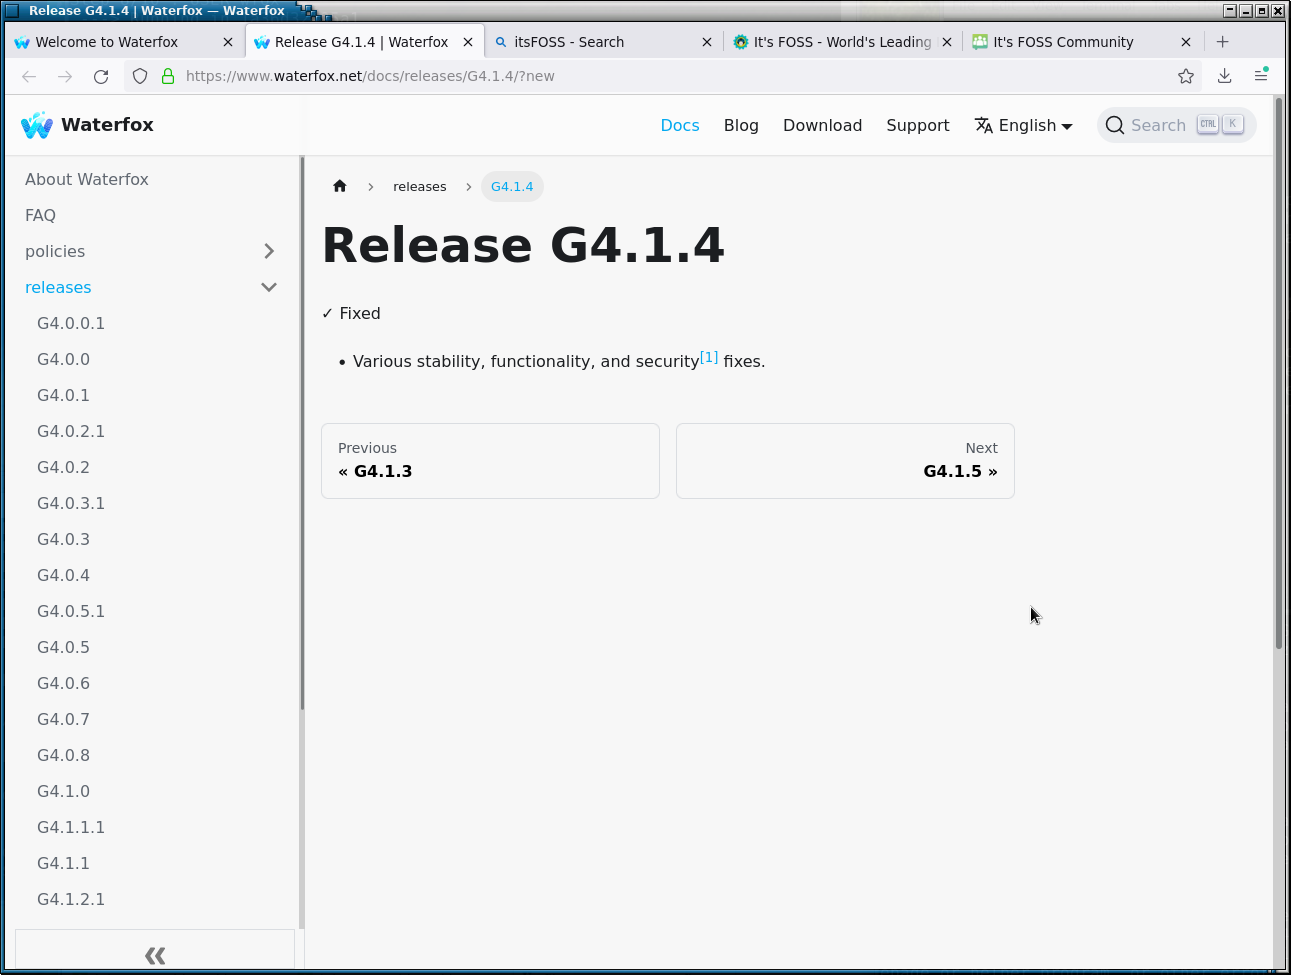
\includegraphics[width=0.9\textwidth]{releas.png}
  \caption{Waterfox Release screen from Dockerfile attempt No 2}
  \label{fig:releas}
\end{figure}

%\end{document}


%\documentclass{article}
%\usepackage{graphicx,subfigure}
%\begin{document}

\begin{figure}[!h]
  \centering
   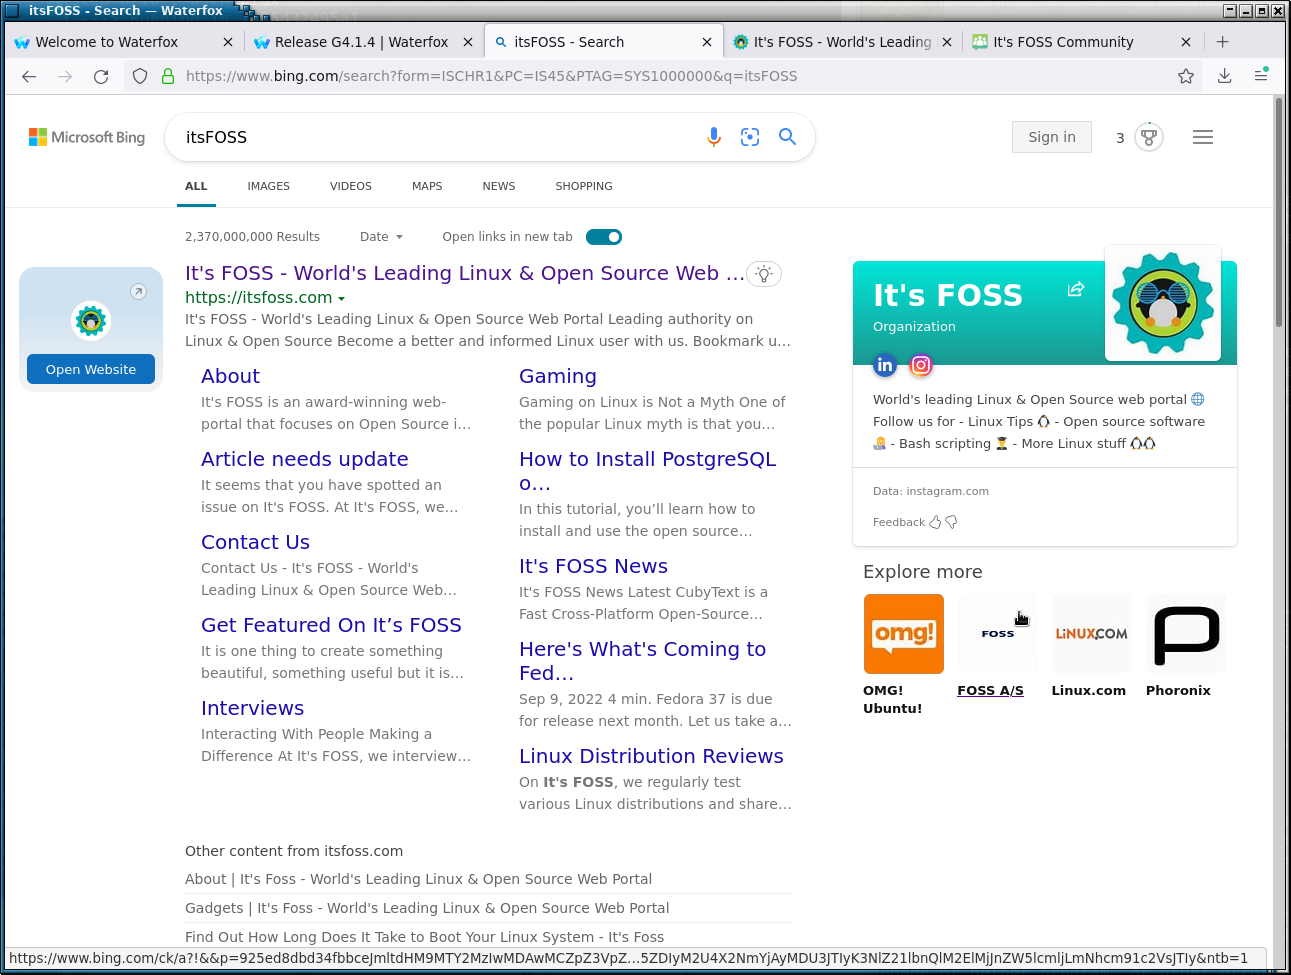
\includegraphics[width=0.9\textwidth]{search.png}
  \caption{Waterfox Google Search screen from Dockerfile attempt No 2}
  \label{fig:search}
\end{figure}

%\end{document}


There are messages in the container terminal as follows
\begin{verbatim}
[nevj@trinity Waterfox.docker]$ docker run -v /tmp/.X11-unix:/tmp/.X11-unix -e DISPLAY=$DISPLAY -h $HOSTNAME -v $HOME/.Xauthority:/home/nevj/.Xauthority wfoxdeb:vt2
Authorization required, but no authorization protocol specified
Unable to init server: Could not connect: Connection refused
Error: cannot open display: :0.0
[nevj@trinity Waterfox.docker]$ xhost +
access control disabled, clients can connect from any host
[nevj@trinity Waterfox.docker]$ 
[nevj@trinity Waterfox.docker]$ docker run -v /tmp/.X11-unix:/tmp/.X11-unix -e DISPLAY=$DISPLAY -h $HOSTNAME -v $HOME/.Xauthority:/home/nevj/.Xauthority wfoxdeb:vt2
Crash Annotation GraphicsCriticalError: |[0][GFX1-]: glxtest: libpci missing (t=0.361222) [GFX1-]: glxtest: libpci missing
Crash Annotation GraphicsCriticalError: |[0][GFX1-]: glxtest: libpci missing (t=0.361222) |[1][GFX1-]: glxtest: libEGL missing (t=0.361261) [GFX1-]: glxtest: libEGL missing
Crash Annotation GraphicsCriticalError: |[0][GFX1-]: glxtest: libpci missing (t=0.361222) |[1][GFX1-]: glxtest: libEGL missing (t=0.361261) |[2][GFX1-]: glxtest: libGL.so.1 missing (t=0.361269) [GFX1-]: glxtest: libGL.so.1 missing
Crash Annotation GraphicsCriticalError: |[0][GFX1-]: glxtest: libpci missing (t=0.361222) |[1][GFX1-]: glxtest: libEGL missing (t=0.361261) |[2][GFX1-]: glxtest: libGL.so.1 missing (t=0.361269) |[3][GFX1-]: glxtest: libEGL missing (t=0.361276) [GFX1-]: glxtest: libEGL missing
Crash Annotation GraphicsCriticalError: |[0][GFX1-]: glxtest: libpci missing (t=0.361222) |[1][GFX1-]: glxtest: libEGL missing (t=0.361261) |[2][GFX1-]: glxtest: libGL.so.1 missing (t=0.361269) |[3][GFX1-]: glxtest: libEGL missing (t=0.361276) |[4][GFX1-]: No GPUs detected via PCI (t=0.361286) [GFX1-]: No GPUs detected via PCI
console.warn: SearchSettings: "get: No settings file exists, new profile?" (new NotFoundError("Could not open the file at /home/wfox/.waterfox/0cuuoqs9.default-default/search.json.mozlz4", (void 0)))
JavaScript error: resource://gre/modules/XPCOMUtils.jsm, line 161: NS_ERROR_XPC_GS_RETURNED_FAILURE: ServiceManager::GetService returned failure code:
JavaScript error: , line 0: InternalError: Promise rejection value is a non-unwrappable cross-compartment wrapper.
JavaScript error: resource://gre/modules/PromiseWorker.jsm, line 106: Error: Could not get children of file(/home/wfox/.waterfox/0cuuoqs9.default-default/thumbnails) because it does not exist
JavaScript error: resource://gre/modules/XULStore.jsm, line 66: Error: Can't find profile directory.
JavaScript error: resource://gre/modules/XULStore.jsm, line 66: Error: Can't find profile directory.
JavaScript error: resource://gre/modules/PartitioningExceptionListService.jsm, line 69: NS_ERROR_MALFORMED_URI: Component returned failure code: 0x804b000a (NS_ERROR_MALFORMED_URI) [nsIPartitioningExceptionListObserver.onExceptionListUpdate]
console.warn: LoginRecipes: "getRecipes: falling back to a synchronous message for:" "https://login.microsoftonline.com"
JavaScript error: https://p.ad.gt/api/v1/p/450, line 1: TypeError: t.vendor is undefined
JavaScript warning: https://pagead2.googlesyndication.com/bg/5BBnFljR3G8Y2LtXULQJm9Fu_0DS9XrGSjZ8CuJ-SSg.js line 2 > eval line 3628 > eval line 1 > eval line 1 > eval, line 1: WebGL warning: <Create>: WebglAllowWindowsNativeGl:false restricts context creation on this system.
JavaScript warning: https://pagead2.googlesyndication.com/bg/5BBnFljR3G8Y2LtXULQJm9Fu_0DS9XrGSjZ8CuJ-SSg.js line 2 > eval line 3628 > eval line 1 > eval line 1 > eval, line 1: Failed to create WebGL context: WebGL creation failed: 
* WebglAllowWindowsNativeGl:false restricts context creation on this system. ()
* Exhausted GL driver options. (FEATURE_FAILURE_WEBGL_EXHAUSTED_DRIVERS)
JavaScript error: , line 0: TypeError: NetworkError when attempting to fetch resource.
console.error: PushService: 
  clearOriginData: Error clearing origin data:
  TypeError
JavaScript error: resource:///modules/Interactions.jsm, line 209: NS_ERROR_FAILURE: Component returned failure code: 0x80004005 (NS_ERROR_FAILURE) [nsIUserIdleService.removeIdleObserver]
JavaScript error: , line 0: TypeError: NetworkError when attempting to fetch resource.
[Parent 7, IPC I/O Parent] WARNING: FileDescriptorSet destroyed with unconsumed descriptors: file /home/ubuntu/actions-runner/_work/Waterfox/Waterfox/ipc/chromium/src/chrome/common/file_descriptor_set_posix.cc:19

###!!! [Child][RunMessage] Error: Channel closing: too late to send/recv, messages will be lost


###!!! [Child][RunMessage] Error: Channel closing: too late to send/recv, messages will be lost

\end{verbatim}
It would seem we have not found all dependencies yet. It says that {\em libpci} and {\em libEGL} are missing, and there are some Javascript resources required.
Instead of just adding those 2 extra libraries/packages, we need to search out why our dependencies searches missed them.

\subsection{Finding missing dependencies after attempt No. 2}

A rerun of all the searches fails to reveal any hint of {\em libpci} and {\
em libEGL} being required. We conclude that some process other than waterfox which runs when the container runs, must be requiring them, perhaps the video drivers?

We can try and see what extra processes are running when the waterfox image is run in a docker container. All tha tcould be found using {\em pa ax} was
\begin{verbatim}
a4170 ?        Sl     0:00 /usr/bin/containerd-shim-runc-v2 -namespace moby -id 33ef059b4edab7b543f72b86d7849df7246d42433ef8d97fb159d7e14d89de4b -address /run/containerd/containerd.sock
 4408 ?        Sl     0:00 /wfox/waterfox/waterfox -contentproc -childID 1 -isForBrowser -prefsLen 1 -prefMapSize 230518 -jsInit 285636 -parentBuildID 20220728185049 -appdir /wfox/waterfox/browser 7 tab
.......   5 more like the above
4488 ?        S      0:00 dbus-launch --autolaunch=796ea3dd4303ebc6c386a3176
4494 ?        Ss     0:00 /usr/bin/dbus-daemon --syslog-only --fork --print-
\end{verbatim}
 So running a container only adds the {\em /usr/bin/containerd-shim-runc-v2} process, and {\em dbus-launch} and {\em dbus-daemon} apart from several processes associates with waterfox.

WE can see what they require
\begin{verbatim}
ldd /usr/bin/containerd-shim-runc-v2
	linux-vdso.so.1 (0x00007fffc3118000)
	libdl.so.2 => /usr/lib/libdl.so.2 (0x00007fb56d758000)
	libpthread.so.0 => /usr/lib/libpthread.so.0 (0x00007fb56d737000)
	libc.so.6 => /usr/lib/libc.so.6 (0x00007fb56d571000)
	/lib64/ld-linux-x86-64.so.2 => /usr/lib64/ld-linux-x86-64.so.2 (0x00007fb56d773000)

ldd /usr/bin/dbus-daemon
	linux-vdso.so.1 (0x00007ffefdb46000)
	libdbus-1.so.3 => /usr/lib/libdbus-1.so.3 (0x00007f8b5d62e000)
	libexpat.so.1 => /usr/lib/libexpat.so.1 (0x00007f8b5d5fd000)
	libpthread.so.0 => /usr/lib/libpthread.so.0 (0x00007f8b5d5dc000)
	libc.so.6 => /usr/lib/libc.so.6 (0x00007f8b5d416000)
	/lib64/ld-linux-x86-64.so.2 => /usr/lib64/ld-linux-x86-64.so.2 (0x00007f8b5d6d3000)

ldd /bin/dbus-launch
	linux-vdso.so.1 (0x00007ffd8226e000)
	libdbus-1.so.3 => /usr/lib/libdbus-1.so.3 (0x00007fc4e7b6a000)
	libX11.so.6 => /usr/lib/libX11.so.6 (0x00007fc4e7a26000)
	libc.so.6 => /usr/lib/libc.so.6 (0x00007fc4e7860000)
	libpthread.so.0 => /usr/lib/libpthread.so.0 (0x00007fc4e783f000)
	libxcb.so.1 => /usr/lib/libxcb.so.1 (0x00007fc4e7814000)
	libdl.so.2 => /usr/lib/libdl.so.2 (0x00007fc4e780e000)
	/lib64/ld-linux-x86-64.so.2 => /usr/lib64/ld-linux-x86-64.so.2 (0x00007fc4e7bdf000)
	libXau.so.6 => /usr/lib/libXau.so.6 (0x00007fc4e7807000)
	libXdmcp.so.6 => /usr/lib/libXdmcp.so.6 (0x00007fc4e77ff000)

\end{verbatim}
but these would be requirements in the host system, not in the waterfox container.
The command {\em docker logs ...} gives the same information as appears in the command line window.  There seems to be no way  to trace the source of these remaining dependencies, which I assume are inside the container.

I tried using {\em strace} on the {\em docker run} statement
\begin{verbatim}
strace docker run -v /tmp/.X11-unix:/tmp/.X11-unix -e DISPLAY=$DISPLAY -h $HOSTNAME -v $HOME/.Xauthority:/home/nevj/.Xauthority wfoxdeb:vt2
execve("/bin/docker", ["docker", "run", "-v", "/tmp/.X11-unix:/tmp/.X11-unix", "-e", "DISPLAY=:0.0", "-h", "trinity", "-v", "/home/nevj/.Xauthority:/home/nev"..., "wfoxdeb:vt2"], 0x7fffd125f8d0 /* 38 vars */) = 0
brk(NULL)                               = 0x308b000
.....
\end{verbatim}
There is  a lot of output,  but the critical messages are the same as appears on the terminal screen.

The only remaining option is to add things by trial and error combined with a touch of intuition.

\subsection{Third Debian parent dockerfile attempt}


\begin{thebibliography}{99}

\bibitem{guru:99}
Docker tutorial.
URL https://www.guru99.com/docker-tutorial.html

\bibitem{dock:00}
Docker get started
URL https://docs.docker.com/get-started/

\bibitem{dock:01}
Docker Desktop
URL https://docs.docker.com/desktop/install/linux-install/

\bibitem{dock:02}
Docker Hub
URL https://hub.docker.com/

\bibitem{dock:03}
Official Dockerfile documnet
URL https://docs.docker.com/develop/develop-images/dockerfile\_best-practices/


\bibitem{dock:04}
Dockerfile Guide
URL https://medium.com/@BeNitinAgarwal/best-practices-for-working-with-dockerfil
es-fb2d22b78186

\bibitem{dock:05}
Docker Basics: How to use Dockerfiles
URL https://thenewstack.io/docker-basics-how-to-use-dockerfiles/

\bibitem{dock:06}
A Beginners Guide to Understanding and Building Docker Images
URL https://jfrog.com/knowledge-base/a-beginners-guide-to-understanding-and-building-docker-images/

\bibitem{dock:07}
Best practices for writing Dockerfiles
URL https://docs.docker.com/develop/develop-images/dockerfile\_best-practices/


\bibitem{dock:09}
Creating a Docke Image for your Application
URL https://www.stereolabs.com/docs/docker/creating-your-image/

\bibitem{dock:10}
Docker Containerization Cookbook” - Hot Recipes for Docker Automation
URL https://distrowatch.tradepub.com/free/w\_java39/prgm.cgi?a=1

\bibitem{void:01}
Void Linux Docker Images
URL https://github.com/void-linux/void-docker


\bibitem{libr:22}
LibreWolf source code website.
URL https://gitlab.com/librewolf-community/browser/source

\bibitem{rehn:21}
Rehn, A. (2021)
Identifying application runtime dependencies: A toolkit for identifying the runtime libraries and associated data that applications require in order to run correctly inside containers. 
URL https://unrealcontainers.com/blog/identifying-application-runtime-dependencies/

\bibitem{wate:22} 
Waterfox website. URL https://www.waterfox.net

\bibitem{wate:22a}
Install the Waterfox browser on a Linux system. URL https://github.com/nevillejackson/Unix/blob/main/waterfox/waterfox.pdf

\bibitem{wate:22b}
WaterfocCo Github site URL https://github.com/WaterfoxCo/Waterfox/releases

\end{thebibliography}
\end{document}
